\documentclass[a4paper,12pt]{article}
\usepackage{amsmath}
\usepackage[utf8x]{inputenc}
%\usepackage{amstext}
\usepackage{graphicx}
\usepackage{color}
\usepackage{array}
\usepackage[left=2cm, top=2cm, right=3cm,
bottom=2cm]{geometry}
%\usepackage[landscape]{geometry}
%\usepackage{lscape}
\usepackage{pdfpages}

\author{Katja Matilainen \\ University of Oulu}
\title{Galaxies \\ Computer assignment for advanced students}
\date{Spring 2016}

\begin{document}

\begin{tiny}
\maketitle
\end{tiny}

\section{The task}
The purpose of this assignment was to study the luminosity profile of the galaxy NGC 7606. To achieve this, an r-band image of the galaxy (file "NGC7606rmosaic.fits"), and iraf scripts "doellipse.cl" and "fixellipse.cl" were provided.

\section{Solution}

\subsection{Ellipticity and position angle}

First, the image was opened with ds9 and all the contaminants (or at least most of them) were masked, and the regions were first saved in CIAO format as "ds9.reg" and then transformed into "NGC7606rmosaic.pl" with the "plcreate" command.

\centerline{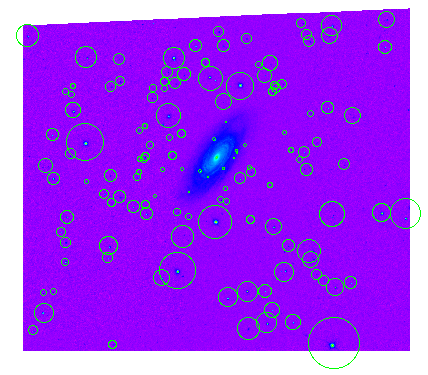
\includegraphics[scale=0.6]{NGC7606.png}}%

Values of the standard deviation of the sky ('STDDEV') were also taken with "imexam" command and saved in a text file for later for error estimating purposes (see example values below).

\centerline{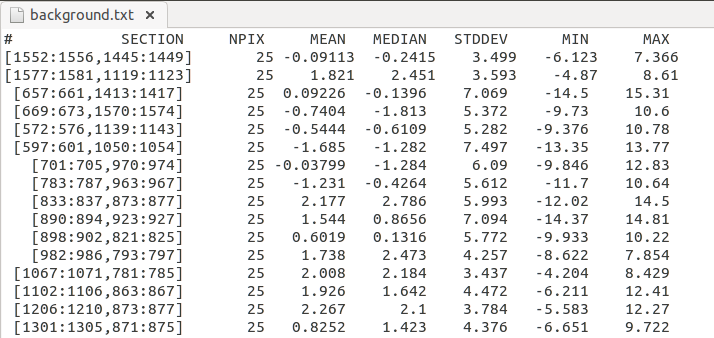
\includegraphics[scale=0.6]{background.png}}%

\vspace*{0.5cm}

These values (about 50 of them) were then combined together with bootstrapping technique to determine the average $\sigma$ value of the sky. The IDL program 'bbootstrap.pro' was downloaded and used for this purpose.

After that the ellipticity and position angle of the galaxy were estimated by using the "doellipse" command in iraf, that fits ellipses of different ellipticity and position angle to the picture. The values of ellipticity, position angle and radius were then read from the file "ell.txt" produced by the iraf script "doellipse.cl", and plotted with IDL. 

In the outskirts of the galaxy, between $r=200-400 \text{px}$ the values were roughly constant, so the final ellipticity and position angle were calculated as an average over that radius (see dashed line in figures 1 and 2 below). After $r>400\text{px}$ radius the fit was no longer reliable, so those values were ignored.

\centerline{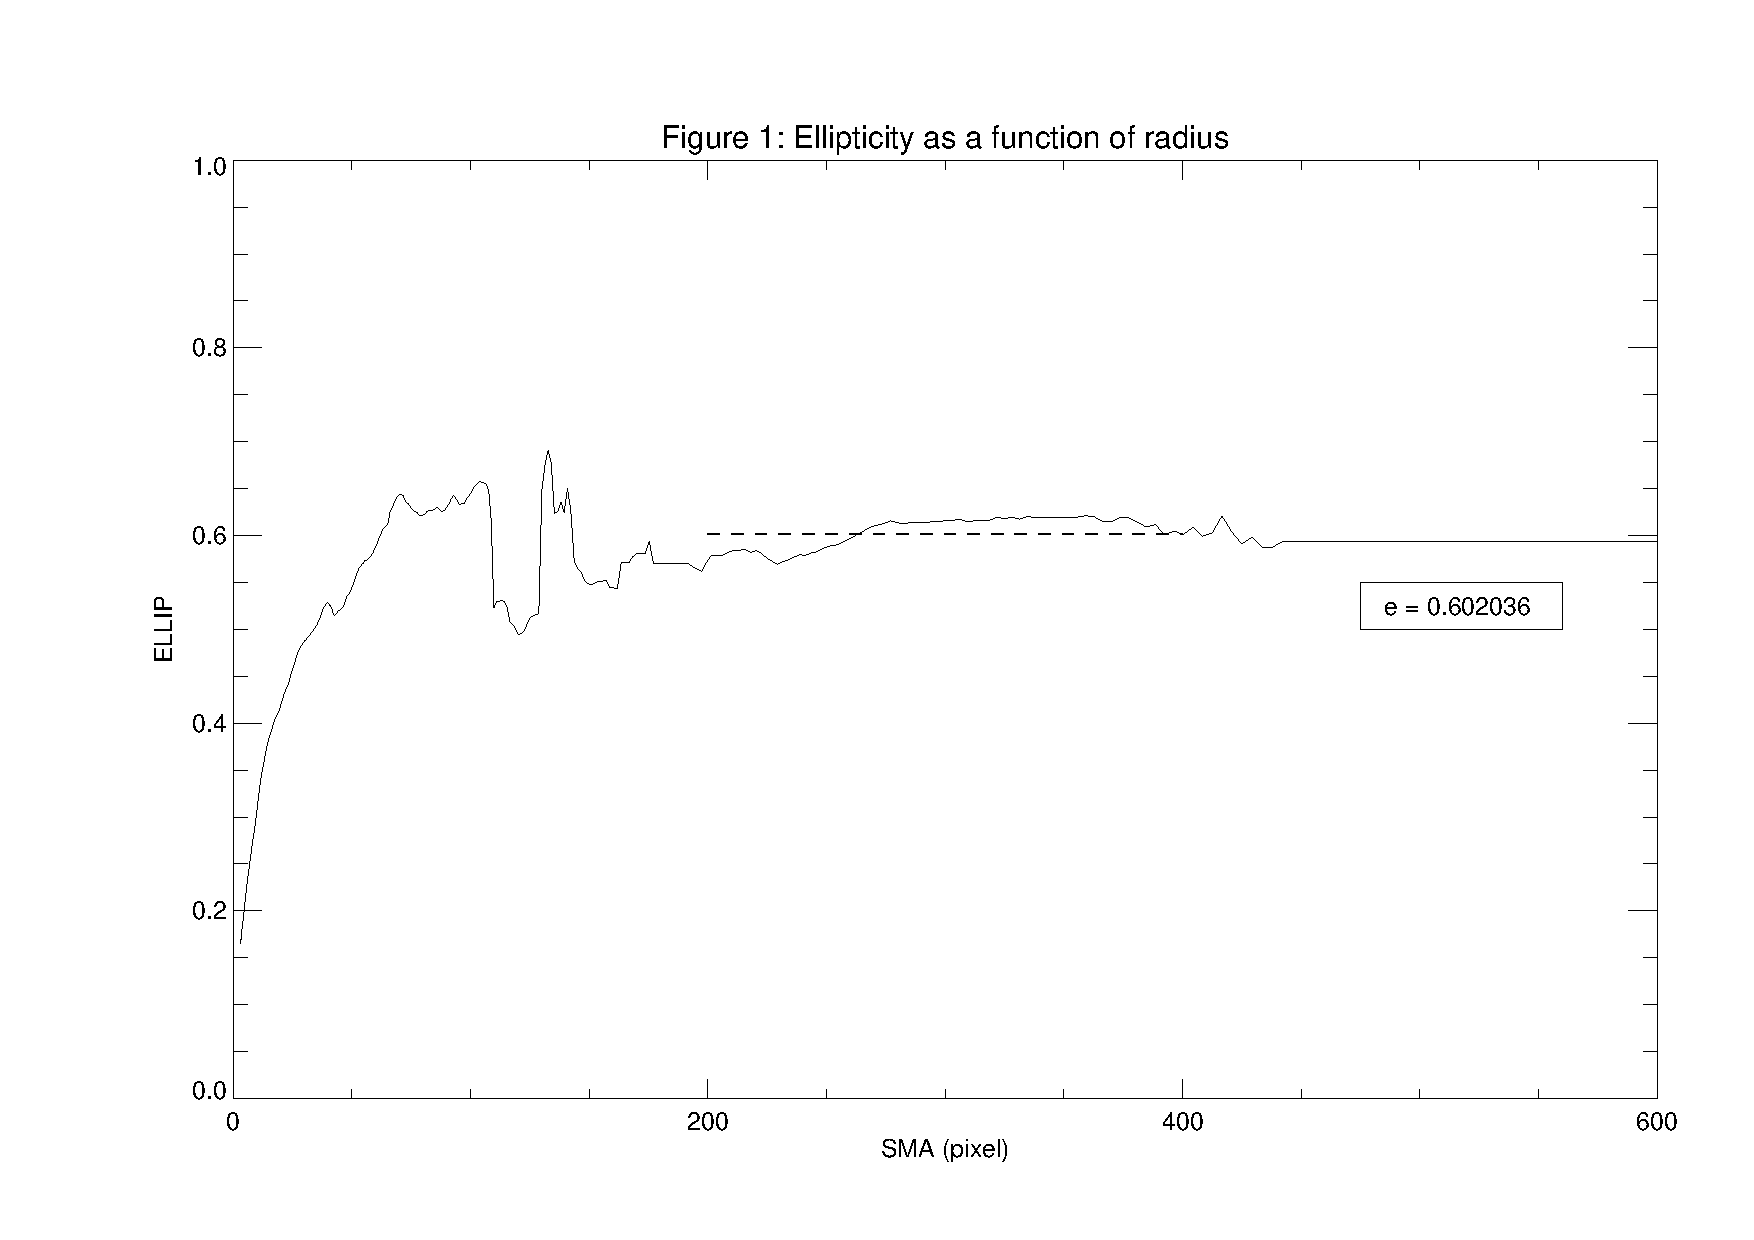
\includegraphics[scale=0.6,page=1]{ellipticity.pdf}}%

\centerline{\includegraphics[scale=0.6,page=2]{ellipticity.pdf}}%

\subsection{Luminosity profile}

The fixed ellipticity and position angle in the outskirts of the galaxy were then used in "fixellipse" command to get the luminosity profile as "ell\_fix.txt". In figure 3 this is presented as intensity as a function of distance from the galactic center in pixels, and in figure 4 the result was converted into magnitudes as a function of radius in arcseconds (one pixel = 0.396 arcseconds). Both plots were again done in IDL.

In figure 4 the error bars were also presented as maximum and minimum magnitudes $M_{max}$ and $M_{min}$ (the dotted lines above and below the original plot). The minimum and maximum values for intensity were first solved from $I_{max}=I+5\sigma$ and $I_{min}=I-5\sigma$, where $\sigma$ is the background value that was determined earlier. The intensities were then transformed into magnitudes with the formula $\mu = -2.5 \log I+26.7713$.

The limiting value for how far from the galactic center the luminosity profile is accurate enough was determined as the radius where $|M-M_{min}|>0.2$, and marked as a vertical line in figure 4.

%μ = −2.5 logI + 26.27713.

\centerline{\includegraphics[scale=0.6,page=3]{ellipticity.pdf}}%

\centerline{\includegraphics[scale=0.6,page=4]{ellipticity.pdf}}%

\subsection{Classification and fitting the final profile of the disk}

The final task was to fit the function
\begin{equation*}
I(R) = S I_0 e^{-\frac{R}{\gamma}} \left[ 1+e^{\alpha (R-R_b)} \right]^{\frac{1}{\alpha}\left(\frac{1}{\gamma}-\frac{1}{\beta}\right)}
\end{equation*}
where
\begin{equation*}
S^{-1}=\left(1+e^{-\alpha R_b}\right)^{\frac{1}{\alpha}\left(\frac{1}{\gamma}-\frac{1}{\beta}\right)}
\end{equation*}
into the luminosity profile to find scale lengths $\gamma$ and $\beta$. 

This was done by using the IDL routine "mpcurvefit.pro" that fits data into a user-submitted function and finds the necessary constants.
For this, the first estimates for $I_0$, $R_b$, $\alpha$, $\beta$ and $\gamma$ were needed. 

First of all, from the luminosity profile it is easily seen that the disk is of Type II, which means that the profile is made of two exponential parts where the inner part is more shallow than the outer one.
The break radius $R_b=106.48440"$ where the steepness changes was roughly estimated by drawing two different lines that touch the luminosity plot, and determining where these lines cross.

From this same picture it was also roughly determined that the bulge of the galaxy ends (and the disk starts) at $R=30"$, which gave the inner limit for the function fitting. The outer limit of the fit was the $R=153.87767"$ that was determined earlier in figure 4. 

(NOTE! This changed to $R=162.69076"$ after changing the ellipticity and position angle, but it's alright to cut the fitting a bit short, since the inner limit was determined only roughly too.)

As for the other constants, alpha was set as $\alpha=0.5/n$, where the initial guess for $n$ was $n=2$. For the scale lengths $\gamma$ and $\beta$ a few test runs with different orders of magnitude were done, and the initial values $\beta=80$ and $\gamma=50$ seemed to give reasonable results.

\centerline{\includegraphics[scale=0.6,page=5]{ellipticity.pdf}}%

%\newpage
In figure 6 the final fitted model is plotted with a dashed line next to the original data.

\centerline{\includegraphics[scale=0.6,page=6]{ellipticity.pdf}}%

After 30 iterations the final values for the constants were

\vspace*{0.5cm}
\centerline{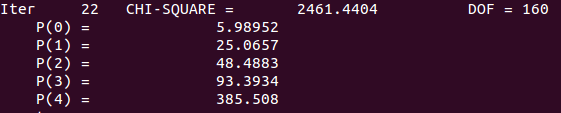
\includegraphics[scale=0.6]{constants.png}}%

which corresponds to

%;const=[n,beta,gamma,sec_b,I0] ;Here sec_b=Rb and alpha=0.5/n
%\begin{center}
%\begin{tabular}{| m{5em} | m{5em} |}
%\hline
$$n = 5.98952$$
$$\alpha = 0.5/n = 0.083479 $$
$$\beta = 25.0657 "$$
$$\gamma = 48.4883 "$$
$$R_b = 93.3934 "$$
$$I_0 = 385.508 \, \text{W}/\text{m}^2$$
%\hline
%\end{tabular}
%\end{center}

If the distance to the galaxy is assumed to be $d=31.78\text{Mpc}$, and we use the relation

$$ \textbf{distance (in pc)} \cdot \textbf{angular size (in ")} = \textbf{actual size (in AU)} $$

the scale lengths become

$$ \beta = 31.78 \cdot 10^6 pc \cdot 25.0657" = 796587946 AU \approx 3862 \text{pc} $$

$$ \gamma = 31.78 \cdot 10^6 pc \cdot 48.4883" = 1540958174 AU \approx 7471 \text{pc} $$

%$$ \beta \approx \frac{25.1355}{60^2}\text{rad} \cdot 31.78 \text{Mpc} = 0.2218906083 \text{Mpc} \approx 220 \text{kpc} $$

%$$ \gamma \approx \frac{48.1847}{60^2}\text{rad} \cdot 31.78 \text{Mpc} = 0.4253638239 \text{Mpc} \approx 430 \text{kpc} $$

%distance 	x 	angular size 	= 	actual size
%(in pc) 		(in as) 		(in AU)

%R b is the
%radius of the break. γ and β are the inner an outer scale-lengths. To transform
%the scale-lengths to kpcs, use d = 31.78 Mpc as the distance to the NGC 7606.

% tan(a)=R/d -> R=d*a



\end{document}